\section{Problem Statement: Bipedal Walker Robot Control}
\label{sec:problem_statement}

\subsection{OpenAI Gym and Bipedal Walker Environment}
\label{ssec:gym_bipedal}

OpenAI Gym \cite{brockman_openai_2016} is open source framework, 
containing many environments to service development of 
reinforcement learning algorithms. 

\textit{BipedalWalker} environments~\cite{noauthor_bipedalwalker-v2_2021, noauthor_bipedalwalkerhardcore-v2_2021} are part of Gym environment library. 
One of them is classical version where the terrain is relatively smooth, while other one is hardcore version which contains ladders, stumps and pitfalls in terrain. 
Those environments have continuous action and observation space. 
For both settings, the task is to move forward the robot as much as possible. 
Snapshots for both environments are in \figref{fig:bipedal_walkers}.
\begin{figure}
	\begin{subfigure}{.5\textwidth}
		\centering
		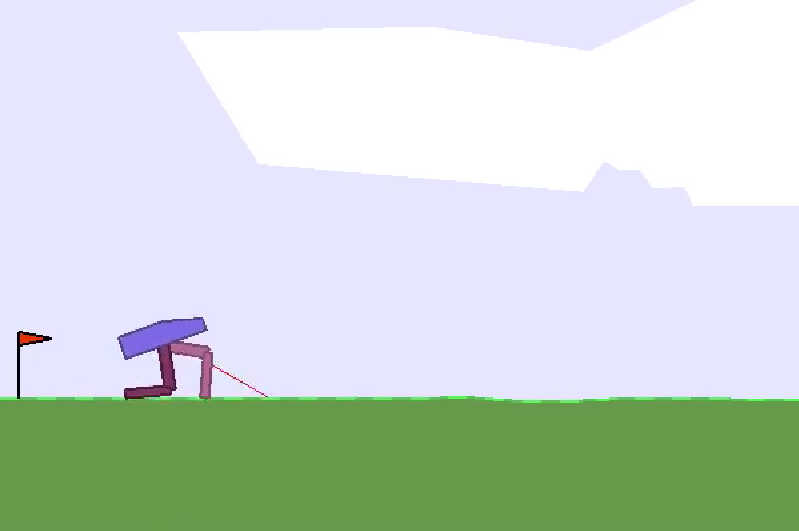
\includegraphics[width=0.9\linewidth]{figures/bipedal/classic.png}
		\caption{BipedalWalker-v3 Snapshot}
		\label{fig:bipedal_walker_classic}
	\end{subfigure}
	\begin{subfigure}{.5\textwidth}
		\centering
		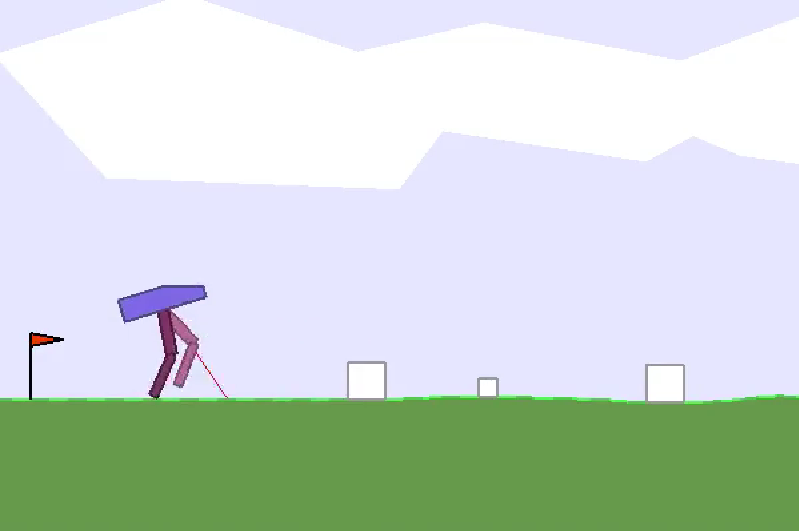
\includegraphics[width=0.9\linewidth]{figures/bipedal/hardcore.png}
		\caption{BipedalWalkerHardcore-v3 Snapshot}
		\label{fig:bipedal_walker_hardcore}
	\end{subfigure}
	\caption{Bipedal Walkers Snapshots}
	\label{fig:bipedal_walkers}
\end{figure}

Locomotion of the Bipedal Walker is difficult control problem due to following reasons. 
\begin{description}
	\item[Nonlinearity] The dynamics are nonlinear, unstable and multimodal. 
	Dynamical behavior of robot changes for different situations 
	like ground contact, single leg contact and double leg concact.
	\item[Uncertainity] The terrain where robot walks may vary. 
	Designing a controller for all types of terrain is difficult.
	\item[Reward Sparsity] Overcoming some obstacles requires a specific maneuver,which is hard to explore sometimes.	
	\item[Partially Observability] The robot observes 
	ahead of it with lidar measurements and cannot observe behind. 
	In addition, it lacks of acceleration sensors.
\end{description}

These difficulties make hard to implement analytical methods for control task. 
RL approach is better to tackle first 2 one. 

Reward sparsity problem brings local minimums to objective function of optimal control. It can be solved by a good exploration strategy and reward shaping. 

For partial observability problem, more elegant solution is required. 
This is done by creating a belief state from past observations to inform agent. 
Agent uses this belief state to choose how to act. 
If belief state is evaluated sufficiently, 
this increases performance of control.
However, relying on observations is also possible for control, 
and this may be enough sometimes if advanced type of control is not required. 

\subsection{Deep Learning Library: PyTorch}
\label{dl_pytorch}
PyTorch is an open source library developed by Facebook's AI Research lab (FAIR)~\cite{paszke_pytorch_2019}. 
It is based on Torch library~\cite{collobert_torch7_2011} and has Python and C++ interface. 
It is an automatic differentation library with accelerated math operations backed by graphical processing units (GPUs). 
This is what a deep learning library requires. 
And the clean pythonic syntax made it most famous deep learning tool among researches. 
